\documentclass[11pt]{article}
\usepackage[a4paper,margin=2.3cm]{geometry}
\usepackage{amsmath,amssymb,bm}
\usepackage{graphicx,booktabs,multirow,xcolor}
\usepackage[authoryear,round]{natbib}
\usepackage[hidelinks]{hyperref}
\usepackage{caption}
\captionsetup{font=small,labelfont=bf}
\newcommand{\pp}{\,pp}

\title{TITLE PLACEHOLDER}
\author{AUTHORS PLACEHOLDER}
\date{Preprint draft, \today}

\begin{document}
\maketitle

\begin{abstract}
ABSTRACT PLACEHOLDER (written after confirmation results).
\end{abstract}

\section{Introduction}

Learning a task that spans hundreds of milliseconds requires assigning credit to synapses whose
influence on behaviour is delayed and passes through recurrent dynamics. The exact solution,
back-propagation through time \citep[BPTT;][]{werbos1990bptt}, needs information that a synapse
does not have: the future error and its path through every other neuron. Local alternatives keep,
at each synapse, an \emph{eligibility trace} of how the synapse could have changed its
postsynaptic cell. They combine it with a broadcast error or reward signal, in line with
three-factor plasticity \citep{gerstner2018}. Examples are RFLO \citep{murray2019rflo} and e-prop
\citep{bellec2020eprop} \citep[see also][]{williams1989rtrl,marschall2020}. These rules are exact
for a cell's own dynamics, and they approximate the rest of the network, for example with random
feedback \citep{lillicrap2016fa}.

What the trace must contain depends on the cell's own dynamics, and real cortical neurons are not
the leaky units used in most such work. Their responses depend on several timescales, and most
show spike-frequency adaptation \citep{benda2003}. For spiking neurons with a single adaptive
threshold, adaptation is known to support memory over behavioural timescales
\citep{bellec2018lsnn,salaj2021sfa}, and e-prop includes the adaptation variable in its
eligibility trace \citep{bellec2020eprop}. Whether this matters for neurons whose intrinsic
dynamics were \emph{fitted to recordings}, with many heterogeneous filters per cell, has been hard
to test: data-fitted single-cell models were usually not differentiable \citep{teeter2018glif}, and
large data-constrained network models have been trained with BPTT
\citep{billeh2020,chen2022v1}. A recent bank of differentiable generalized firing-rate (GFR)
models, fitted to more than a thousand patch-clamp recordings \citep{yeung2025gfr}, now makes the
test possible.

We built recurrent networks entirely from these fitted cells, keeping each cell's intrinsic
parameters frozen and making only the synaptic weights plastic. We asked three questions:
(i) how close a cell-local, forward-in-time rule comes to the exact gradient on working-memory
tasks, compared with a frozen recurrent reservoir; (ii) whether the rule must include each cell's
fitted spike-history filter in its eligibility trace; and (iii) whether the specific identity of
the cells (the natural pairing of each cell's parameters and their heterogeneity) or the type-based
wiring matters for learning, once confounds are removed.

The third question carries a trap that we found in our own earlier analyses. Shuffling parameters
across cells moves each cell away from the operating point it was calibrated to. In our networks
this roughly doubled firing rates and multiplied saturation, so an apparent effect of
``destroying biological identity'' could not be separated from a change of operating point. We therefore
recalibrate every manipulated bank with the same label-free procedure before comparing. We also
split cells by donor animal, compare learners at learning rates tuned on a separate development
cohort, treat the network as the unit of inference \citep{aarts2014}, fit every population-analysis
axis on trials independent of those it is evaluated on \citep{kriegeskorte2009}, and test all
hypotheses in a protocol locked before the held-out confirmation cohort was touched.

Four things came out of the held-out confirmation (1,680 networks).
\begin{itemize}
\item The local rule needs each cell's fitted spike-history term. Without it, accuracy at unseen
delays dropped by 7--17\pp, to about the level of a frozen reservoir. With it, the local
estimate stayed aligned with the exact gradient, and the gain grew with each cell's adaptation
strength.
\item The local rule still trails BPTT on tasks that combine memory with a later cue. The gap
comes from ignoring paths through other cells, not from random feedback.
\item Cell identity and type-level wiring had no detectable effect once operating points were
matched. Heterogeneity helped BPTT strongly but not the local rule.
\item The operating point shaped local learning in a task-dependent way.
\end{itemize}

\section{Results}
RESULTS PLACEHOLDER (filled from the confirmation cohort).

\section{Discussion}

We trained recurrent networks made entirely of data-fitted neuron models with a cell-local,
forward-in-time learning rule, and tested every comparison in a protocol locked before the
held-out cohort was used. Four results stand out.

\paragraph{The eligibility trace must contain the fitted adaptation.}
Almost every fitted cell adapts. A local rule whose eligibility trace ignores the cell's own
spike-history filter lost 7--17\pp of out-of-distribution accuracy and fell to the level of a
frozen reservoir. The reason is credit assignment: with $\beta$, the local estimate stays
closely aligned with the exact gradient (cosine up to 0.94 with symmetric feedback), and the
benefit is larger at cells with stronger adaptation loop gain. This extends a point made for
single-threshold adaptive spiking neurons
\citep{bellec2020eprop,bellec2018lsnn,salaj2021sfa}: it holds for heterogeneous, multi-timescale
history filters fitted to real cells. For a synapse, the requirement is concrete. Its trace
must decay with the postsynaptic cell's own adaptation kinetics, not only with membrane or
synaptic time constants.

\paragraph{Where local learning falls short.}
On the two tasks that require combining stored information with a later cue, the local rule
trailed BPTT by 11--22\pp. Symmetric feedback did not close that gap, which points to the paths
through other cells that the rule ignores, rather than to random feedback. The frozen reservoir
was a strong baseline. Population codes show why: the slow fitted filters keep both input
streams decodable through the delay in every network, so learning matters mainly in the response
phase. A frozen reservoir is therefore the right control for claims about recurrent plasticity in
networks of slow cells; in our data, local plasticity beat it significantly in half of the
comparisons.

\paragraph{Biological specificity: a negative result with one exception.}
Once each manipulated bank was recalibrated to the same operating point, the natural pairing of
each cell's parameters and the type-level wiring had no detectable effect. Most such effects
were bounded within $\pm$5\pp. Without recalibration, shuffled networks ran at twice the rate
with about 15 times more saturation. That is a different regime, and earlier versions of this
project had read differences between such networks as effects of cell identity. Heterogeneity
was the exception. Replacing cells by their type means cost BPTT up to 25\pp on the harder tasks,
in line with reports that heterogeneity aids learning \citep{pereznieves2021}, but it did not
affect the local rule. One possible reading is that the diversity of timescales is only useful
to a learner that can assign credit through the network. A local rule that cannot do so does not
benefit from it. Type-mean networks also fired more slowly, so part of this effect may be an
operating-point difference that our calibration did not remove.

\paragraph{Operating point.}
The calibrated baseline rate, a choice that every data-constrained rate model makes, mattered
for the local rule in a task-dependent way and not for BPTT. It should be reported and
varied, not fixed silently.

\paragraph{Limitations.}
\begin{itemize}
\item \emph{The models are rate models.} The GFR models reproduce each cell's firing-rate
response, not spikes, dendrites or conductance-based synapses. The adaptation we find to matter
is the fitted rate-history filter. Spike-level adaptation mechanisms are not modelled.
\item \emph{The cells and the tasks come from different areas.} The cells are mostly from mouse
visual cortex, and the tasks are abstract working-memory tasks. We make no claim that these
circuits solve these tasks in vivo.
\item \emph{The wiring is a prior, not data.} Type-level connection probabilities are modelling
assumptions (Table~\ref{tab:priors}). Measured probabilities were not used because the numbers
we could trace were available only as figures.
\item \emph{The fits have a known split caveat.} Upstream, one stimulus protocol contributes to
both fitting and validation. We selected cells on the released validation criterion and claim no
new patch-clamp validation.
\item \emph{Optimization is a confound we only bound.} Adam with global clipping is not local. We
therefore repeated every learning-rule comparison with per-synapse RMS normalization, which is
local, but no optimizer is a model of biological plasticity. The local rule also uses a
broadcast error and fixed random feedback; we did not test reward-based or neuromodulatory
variants.
\item \emph{Scale.} Networks have 100 cells, with 16 paired seeds per condition. Each network uses
80 of 170 pyramidal cells, so networks share cells: inference is about networks built from this
cohort, not about new cells.
\item \emph{The operating point is a modelling choice.} Calibrating every cell to a fixed fraction
of its own ceiling sets the type-specific rate hierarchy by construction. Family D shows how much
results depend on this choice.
\end{itemize}


\paragraph{Outlook.}
The same pipeline can test spiking versions of the fitted cells, measured connectivity once it
is available in tabular form, reward-modulated rather than supervised signals, and larger
networks. The protocol, code and all run outputs are available for reuse.

\section{Methods}\label{sec:methods}

\subsection{Data-fitted neuron models}
We used the differentiable generalized firing-rate (GFR) models of \citet{yeung2025gfr}.
They were fitted to whole-cell current-clamp recordings in the Allen Cell Types Database
\citep{gouwens2019}, and we took the code and data from upstream commit \texttt{835a535}. Each
cell $i$ has $K=8$ filters with fixed time constants
$\tau_k\in\{{\approx}0, 20, 50, 100, 200, 500, 1000, 2000\}$\,ms. At the fitted bin size
$\Delta t=20$\,ms the decay coefficients are $d_k = 1-e^{-\Delta t/\tau_k}$, shared by all cells.
With input current $I_{i,t}$ (pA) and rate $r_{i,t}$ (Hz),
\begin{align}
h^{(k)}_{i,t} &= (1-d_k)\,h^{(k)}_{i,t-1} + a_{ik}\,I_{i,t} + \beta_{ik}\,r_{i,t-1},\label{eq:gfr-h}\\
r_{i,t} &= \gamma_i\,\mathrm{ReLU}\!\Big[\tanh\Big(\textstyle\sum_{d}c_{id}^2\,x_{i,t}^{\,d}\Big)\Big],
\qquad x_{i,t}=\big(\bar h_{i,t}-b_i\big)/\sigma_i,\quad \bar h_{i,t}=\tfrac1K\textstyle\sum_k h^{(k)}_{i,t}.\label{eq:gfr-r}
\end{align}
The stored $a_{ik}$ and $\beta_{ik}$ already include the discretization, so no extra $\Delta t$
factor is applied. Upstream rates in spikes/ms are converted to Hz once. Fitted parameters are
never changed by training. Our implementation reproduces the upstream equation for all 1,124
fitted cells (unit tests).

The coefficients $\beta_{ik}$ form the cell's spike-history filter. Its steady-state gain
$\bar\beta_i=\tfrac1K\sum_k\beta_{ik}/d_k$ (pA\,Hz$^{-1}$) is negative for almost every cell,
which is spike-frequency adaptation \citep{benda2003,weber2017glm}: median $-10.5$ for pyramidal
(Pyr) cells, $-6.6$ for SST, $-4.1$ for VIP and $-0.8$ for PV cells in the development cohort.

\paragraph{Cells and cohorts.}
Following the upstream release criterion, we kept mouse cells with validation explained
variance $\ge0.5$. We did not select on the held-out test sweeps. Operational labels came from
Cre line and dendrite type: spiny cells from excitatory lines are Pyr, and Pvalb-, Sst- and
Vip-Cre cells are PV, SST and VIP. This gave 597 cells (339 Pyr, 107 PV, 86 SST, 65 VIP) from 410
donors, mostly in primary visual cortex. Whole donors were assigned to a development cohort (298
cells) or a confirmation cohort (299 cells). The assignment was a seeded, type-stratified greedy
procedure. No donor contributes to both cohorts. All tuning and piloting used only the development
cohort.

\subsection{Networks}
A network has $N=100$ cells, 80 Pyr, 10 PV, 5 SST and 5 VIP, sampled without replacement for each
network seed. The input current to cell $i$ is
\begin{equation}
I_{i,t}=I^0_i + S_i\Big(\textstyle\sum_c W^{\rm in}_{ic}u_{c,t}+\sum_j s_j |W_{ij}| M_{ij}\, r_{j,t-1}/R_0\Big),
\end{equation}
with $R_0=100$\,Hz for every cell. The sign $s_j$ is $+1$ for Pyr and $-1$ for interneurons
(Dale's law). The mask $M$ is drawn from a type-level connection-probability matrix inspired by
cortical motifs \citep{pfeffer2013,pi2013}. These are modelling assumptions, not measured values
(Table~\ref{tab:priors}). Magnitudes $|W_{ij}|$ are log-normal with mean 1 ($\sigma_{\log}=0.35$),
scaled by $0.6/\langle\text{in-degree}\rangle$, and inhibitory sources are multiplied by 1.5.
Input weights are $W^{\rm in}_{ic}\sim\mathcal N(0,1/5)$. The readout
$z_t=\sum_{i\in\rm Pyr}w_i r_{i,t}/R_0+b$ uses Pyr cells only.

\paragraph{Operating-point calibration.}
For each cell, $I^0_i$ is chosen on a 33-point grid in $[0,\sigma_i]$ so that its isolated
steady-state rate is closest to 5\% of its own fitted ceiling $\gamma_i$. The rate is measured in
the last third of a 3-s constant-current probe. The input scale is $S_i=0.25\,\sigma_i$. The
procedure uses no task information. Because the target is relative to each cell's ceiling, the
resulting baseline rates differ by type (PV higher), by construction.

\paragraph{Identity and wiring controls.}
\emph{Within-type shuffle}: independent permutations, within each type, of the input filters
$a_{i\cdot}$, the history filters $\beta_{i\cdot}$ and the activation tuple
$(\sigma,\gamma,c,b)$. This keeps marginal distributions and breaks the pairing of a cell's own
parameters. \emph{Type-homogeneous}: every parameter is replaced by its type mean.
\emph{Cross-type permutation}: whole parameter tuples are permuted across types. \emph{Fast
decay}: $d_k\leftarrow\max(d_k,1-e^{-1})$, so $\tau_k\le20$\,ms, with $a$ and $\beta$ rescaled to
keep $a/d$ and $\beta/d$, and hence the static response. Unless stated otherwise, each manipulated
bank is recalibrated with the same label-free procedure (``matched''). The ``reference''
calibration keeps the intact bank's $I^0,S$, as in earlier versions of this project; it is shown as
a control. \emph{Degree-preserving rewiring} applies $10|E|$ directed double-edge swaps. It
preserves every cell's in- and out-degree, its Dale sign and its multiset of outgoing magnitudes.

\subsection{Tasks}
Inputs have five channels: two sensory streams (A, B), two cue channels and a go signal. Time is
binned at 20\,ms: fixation 100\,ms, stimulus 200\,ms, a silent delay of 100, 200 or 300\,ms in
training, and a 60-ms response window marked by the go channel. Sensory evidence has signed
coherence $\pm\{0.25,0.5,1\}$ plus Gaussian noise ($\sigma=0.25$ per bin). Every batch is exactly
balanced over cue, relevant sign and irrelevant sign.
\emph{T1-early} \citep[context-dependent decision;][]{mante2013}: a context cue during fixation and
stimulus says which stream is relevant, and the target is the sign of the relevant stream.
\emph{T1-late}: the same, but the context cue (60\,ms) arrives only after the delay, so both
streams must be held. \emph{T2-dms} (delayed match-to-sample, \citealp{miller1996,masse2019}):
stream A is the sample and stream B a simultaneous distractor. A $\pm1$ probe arrives after the
delay, and the target is $\mathrm{sign(sample)}\times\mathrm{probe}$, so no input before the probe
carries information about the choice. Conflict trials are those whose two streams have opposite
signs. Test splits are 512 trials each: in-distribution (ID); unseen delays of 400 and 600\,ms
(OOD); higher sensory noise ($\sigma=0.5$); a 40-ms zero-mean distractor ($\sigma=0.75$) in
mid-delay; and all three combined.

\subsection{Loss and learning rules}
The loss is the binary cross-entropy of $z_t$ at every response bin, averaged within a trial and
then over the batch. The choice is the sign of the mean response-window logit. Only $|W|$ (masked,
non-negative, at most 2), $w$ and $b$ are plastic.

\paragraph{BPTT.} The exact gradient by back-propagation through time \citep{werbos1990bptt}
through all filters, the spike-history loop and the recurrent connections. It was checked against
central finite differences.

\paragraph{Local rule.} The local rule is e-prop \citep{bellec2020eprop}, which is related to
RFLO \citep{murray2019rflo}, adapted to GFR cells. It approximates $\partial\mathcal L/\partial
W_{ij}$ by
\begin{equation}
\hat g_{ij}=\sum_t L_{i,t}\,\frac{g'_{i,t}}{R_0}\,\bar e_{ij,t},\qquad
L_{i,t}=B_i\,\frac{\partial \mathcal L}{\partial z_t},
\end{equation}
where $B$ is a fixed random feedback vector \citep{lillicrap2016fa} and $g'$ is the activation
slope. The $K$-dimensional eligibility trace $e_{ij,t}=\partial h_{i,t}/\partial W_{ij}$ follows
only cell $i$'s own dynamics, with presynaptic activity held fixed:
\begin{equation}
e^{(k)}_{ij,t}=(1-d_k)\,e^{(k)}_{ij,t-1}+a_{ik}S_i s_j\,\frac{r_{j,t-1}}{R_0}
+\underbrace{\beta_{ik}\,g'_{i,t-1}\,\bar e_{ij,t-1}}_{\text{spike-history term}}.\label{eq:elig}
\end{equation}
Every quantity is available at the synapse or the postsynaptic cell, plus one broadcast error
signal \citep{gerstner2018}. \emph{No-$\beta$} removes only the spike-history term in
Eq.~\ref{eq:elig}; the network dynamics are unchanged. \emph{Symmetric feedback} uses $B=w$ (the
readout weights), which isolates the error introduced by ignoring paths through other cells. The
quantity in Eq.~\ref{eq:elig} can be computed forward in time, as a synapse would, or by an
equivalent reverse sweep over each cell's own dynamics, which is the network gradient with all
paths through other cells removed. The two agree to $<10^{-10}$ relative error (unit tests). We
used the reverse sweep because it is $\sim$17$\times$ faster.

\paragraph{Frozen reservoir.} Recurrent weights are fixed, and only $w,b$ are trained, with their
exact gradient.

\paragraph{Optimizers.} \emph{Adam} \citep{kingma2015adam} with global gradient-norm clipping at
1.0 is the primary optimizer. \emph{RMS} is per-parameter RMS normalization without momentum and
without clipping \citep{tieleman2012rmsprop}, so every update depends only on that synapse's own
history. It is an optimizer, not a model of homeostatic synaptic scaling \citep{turrigiano2008}.
After each update, magnitudes are projected onto $[0,2]$.

\paragraph{Training and model selection.} Each run trains for 3000 updates of 32 trials.
Validation uses 256 ID trials every 50 updates, and the checkpoint with the lowest validation BCE
(including the untrained network) is kept. Learning rates were chosen on the development cohort
only. The grid was $\eta_{\rm rec}\in\{3\cdot10^{-4},10^{-3},3\cdot10^{-3},10^{-2}\}\times
\eta_{\rm out}\in\{0.03,0.1,0.3,1\}$, three seeds per candidate, and the criterion was mean best
validation BCE. This was done separately for each learner, task and optimizer
(Table~\ref{tab:lr}). A second stage tried $\eta_{\rm out}\in\{3,10\}$ at each learner's
selected $\eta_{\rm rec}$, because with Adam the frozen reservoir and the no-$\beta$ rule were
still improving at the top of the grid. The final choice minimized the same criterion over both
stages; the reservoir's optimum ($\eta_{\rm out}=3$) is then inside the range tried. An earlier
search with $\eta_{\rm out}\le0.1$ had put every learner at its upper edge and was discarded. No
test split had been evaluated at any of these points. Controls use the rates of their learner. A network seed fixes the sampled
cells, graph, initial weights, feedback vector and every trial, so all conditions are paired.

\subsection{Analyses}
\paragraph{Population codes.} For each phase (stimulus, delay, response), we fitted PCA, ridge
probes ($\alpha=1$) for choice, cue and each stream's sign, and a class-mean choice axis on 128
\emph{analysis-fit} trials. All were evaluated on 128 independent \emph{analysis-evaluation}
trials, to avoid double dipping \citep{kriegeskorte2009}.

\paragraph{Gradient alignment.} At each saved checkpoint, on 32 independent diagnostic trials, we
computed the cosine between the exact recurrent gradient and each local estimate: with or without
$\beta$, and with random or symmetric feedback. Per-neuron alignment uses the row of the gradient
belonging to postsynaptic cell $i$. Each cell's \emph{adaptation loop gain} is
$|\langle g'_i\rangle\,\bar\beta_i|$, the steady-state history gain times the mean activation
slope on those trials.

\subsection{Statistics and protocol}
The unit of inference is the network. We avoid pooling cells or trials as if they were
independent \citep{aarts2014}. Comparisons are paired by seed and use exact two-sided sign-flip
tests over all $2^{16}$ sign assignments, with percentile bootstrap CIs over networks. Families of
tests and the Holm correction are as preregistered (Section~\ref{sec:protocol}). The 2$\times$2$\times$2
factorial effects (identity, wiring, learner) are main effects and interactions computed within
each network. An identity, wiring or heterogeneity effect is called \emph{practically negligible}
when its 90\% CI lies within $\pm5$\pp. The protocol, the analysis code and the source hash were
locked before the confirmation cohort was used (Supplementary Section~\ref{sec:protocol}). Results
outside it are labelled exploratory.


\section*{Code and data availability}
All code, configurations, the locked protocol and every run's raw outputs (per-trial
predictions, learning curves, checkpoints) are in the project repository. The fitted
neuron models and cell metadata are those released by \citet{yeung2025gfr}
(AllenInstitute/GRNN, commit \texttt{835a535}) under their original licence.

\bibliographystyle{abbrvnat}
\bibliography{refs}

\clearpage
\appendix
\section{Supplementary information}

\subsection{Locked protocol}\label{sec:protocol}
The confirmatory protocol (\texttt{docs/PREREGISTRATION\_v11.md}) fixed the cohorts, network,
tasks, training budget, learning-rate selection, conditions, endpoints, test families and
equivalence margin before any confirmation-cohort run. Its SHA-256, the source-code hash and the
analysis-script hash are recorded in \texttt{docs/LOCK\_v11.json} (Table~\ref{tab:lock}).

\begin{table}[h]\centering\small\caption{Protocol lock record.}\label{tab:lock}
\begin{tabular}{ll}\toprule
locked at utc & \texttt{2026-11-08T20:23:06.054737+00:00}\\
protocol sha256 & \texttt{34453091eb6167c1fcb563b9edb4ee73...}\\
source hash & \texttt{6f3ff264daccfdeee2dae6656539f3bf...}\\
analysis sha256 & \texttt{705004bdb741278852253c48243748dd...}\\
confirmation configs sha256 & \texttt{ecadfeb93d31af97f7390359925c76a1...}\\
\bottomrule\end{tabular}\end{table}


\subsection{Connection-probability prior}
\begin{table}[h]\centering\small
\caption{Type-level connection probabilities $P(\text{target}\leftarrow\text{source})$ used to
draw the recurrent mask. They are modelling assumptions inspired by
\citet{pfeffer2013,pi2013}, not measurements for the sampled cells.}\label{tab:priors}
\begin{tabular}{lcccc}\toprule
target $\backslash$ source & Pyr & PV & SST & VIP\\ \midrule
Pyr & 0.20 & 0.50 & 0.45 & 0.05\\
PV  & 0.45 & 0.35 & 0.30 & 0.05\\
SST & 0.35 & 0.05 & 0.05 & 0.70\\
VIP & 0.30 & 0.05 & 0.40 & 0.05\\ \bottomrule
\end{tabular}\end{table}

\subsection{Selected learning rates}
\begin{table}[h]\centering\small
\caption{Learning rates selected on the development cohort by validation BCE (recurrent / readout). The frozen reservoir has no recurrent rate.}\label{tab:lr}
\begin{tabular}{llcccc}\toprule
task & optimizer & BPTT & local & local (no $\beta$) & reservoir\\ \midrule
early & adam & 0.001 / 1 & 0.003 / 3 & 0.001 / 3 & -- / 3\\
early & rms & 0.001 / 10 & 0.003 / 0.3 & 0.0003 / 0.3 & -- / 0.3\\
late & adam & 0.003 / 1 & 0.001 / 3 & 0.001 / 1 & -- / 3\\
late & rms & 0.003 / 3 & 0.001 / 1 & 0.003 / 0.3 & -- / 0.3\\
dms & adam & 0.003 / 1 & 0.003 / 1 & 0.001 / 1 & -- / 3\\
dms & rms & 0.003 / 0.1 & 0.001 / 1 & 0.003 / 0.3 & -- / 0.3\\
\bottomrule\end{tabular}\end{table}


\subsection{Supplementary figures}
\begin{figure}[h]\centering
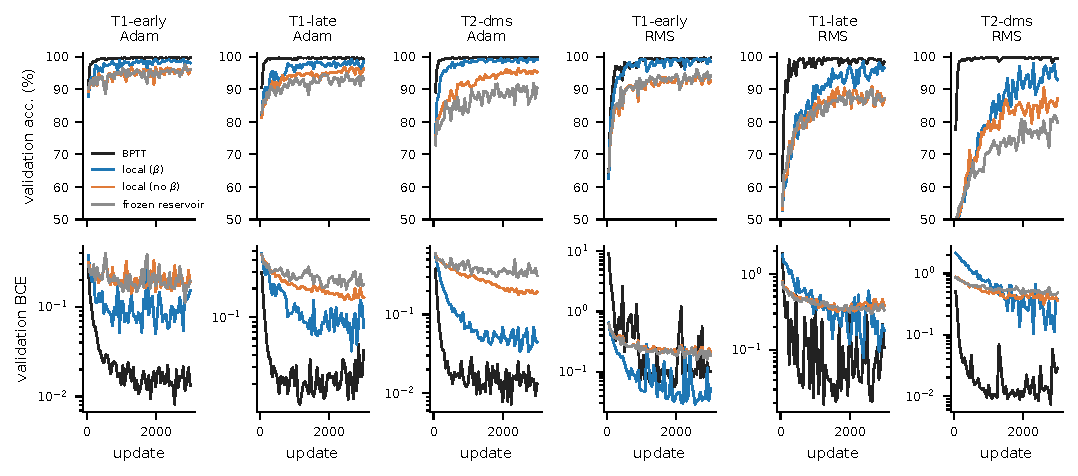
\includegraphics[width=\textwidth]{figures/figS1_learning_curves.pdf}
\caption{\textbf{Validation learning curves} (in-distribution trials; mean over 16 confirmation
networks) for each learner, task and optimizer. Accuracy saturates early, and validation BCE keeps
falling for all learners.}\label{fig:s1}
\end{figure}
\begin{figure}[h]\centering
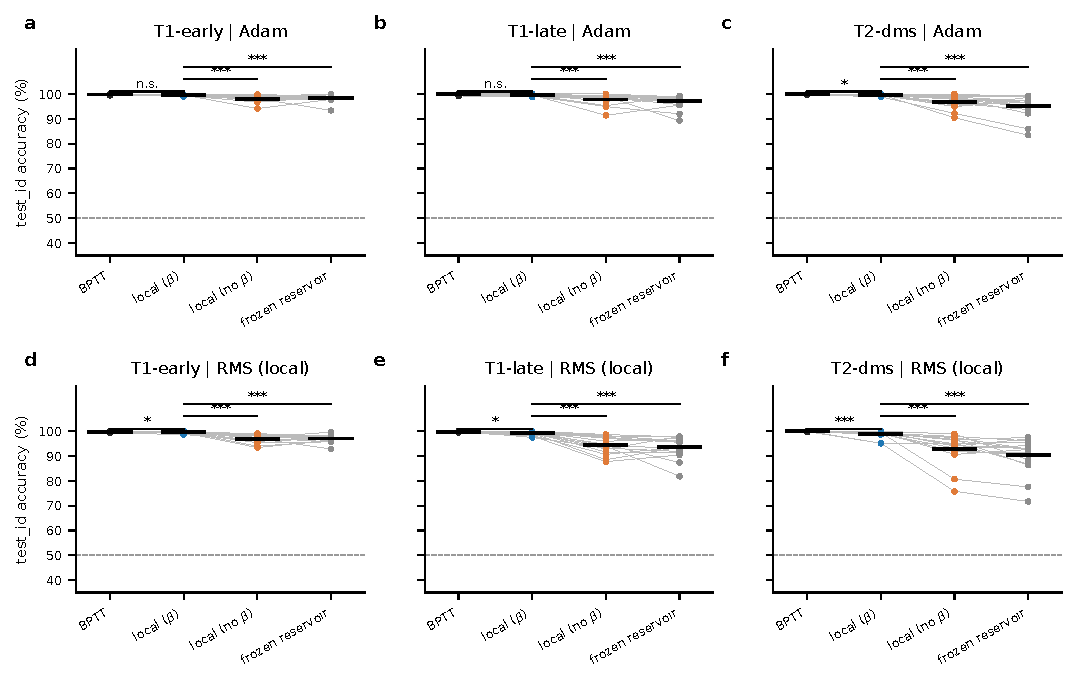
\includegraphics[width=\textwidth]{figures/figS2_id_accuracy.pdf}
\caption{\textbf{In-distribution accuracy} (training delays) for the learners of
Fig.~\ref{fig:rules}. Every learner is near ceiling, which is why the preregistered endpoint uses
unseen delays. Brackets show the same contrasts on this secondary endpoint (Holm within that
endpoint).}\label{fig:s2}
\end{figure}

\subsection{Relation to earlier versions of this project}
Earlier internal versions compared intact and shuffled cells while keeping the intact bank's
calibration. They split cells by specimen (65 donors were shared between cohorts), compared
learners after a fixed short budget at which none had converged, and used one task. Those
results are not used here. All numbers in this paper come from the runs described in
Methods.

\end{document}
